\section{Hardware Setup and Oscilloscope Capture}
\label{app:hw}

\subsection{Board Comparison}

\begin{table}[H]
\centering
\caption{All boards evaluated in this project.}
\begin{tabular}{@{}p{4.2cm}p{3.5cm}p{2.3cm}p{4cm}@{}}
\toprule
Board & MCU & Outcome & Root cause \\
\midrule
Raspberry Pi Pico & RP2040, Cortex-M0+, 125\,MHz & Failed &
  On-chip SMPS ($\approx$1\,MHz switching noise on DVDD) \\
Arduino Uno R4 Minima & Renesas RA4M1, Cortex-M4, 48\,MHz & Failed &
  Internal DC-DC regulation + only 2{,}000 traces \\
\textbf{Adafruit Pro Tinkrer 5\,V} & \textbf{ATmega328P, 16\,MHz} &
  \textbf{Success} & Clean 5\,V linear supply; no SMPS \\
\bottomrule
\end{tabular}
\end{table}

\subsection{Pro Tinkrer 5\,V @ 16\,MHz Setup}
\label{app:hw:trinket}

\textbf{Target:} Adafruit Pro Tinkrer 5\,V 16\,MHz~\cite{adafruit_trinket_pro}
(ATmega328P~\cite{atmega328p}, same MCU as the classic Arduino Uno).

\subsubsection*{Wiring Diagram}

\begin{verbatim}
USB 5V ----+---- [10 Ohm shunt] ----+---- Pro Tinkrer VCC pin
           |                        |
           |              [scope CH1+]  <- Keysight oscilloscope (differential)
           |              [scope CH1-] -- GND
           |
           +-- GND -------------------------------- Trinket GND pin

Trigger:
  Trinket GPIO 8 ----------- scope CH2 / EXT TRIG BNC (rising edge)

Host serial:
  USB-UART adapter (FTDI) -- /dev/tty.usbserial-XXXX
  Trinket TX/RX ------------ adapter RX/TX
  Baud: 115200
\end{verbatim}

% TODO-SCHEMATIC-FIGURE: Replace the text diagram above with a proper figure.
% Suggested path: report/figures/trinket_schematic.png
% Uncomment and fill in once the image is ready:
%
% \begin{figure}[H]
%   \centering
%   \includegraphics[width=0.85\linewidth]{figures/trinket_schematic.png}
%   \caption{Pro Tinkrer 5\,V measurement setup schematic. 10\,$\Omega$
%            shunt on VCC rail; GPIO\,15 trigger to scope CH2.}
%   \label{fig:schematic}
% \end{figure}

\subsubsection*{Oscilloscope Settings}

\begin{itemize}
  \item \textbf{Model:} Keysight / Agilent oscilloscope\\
        VISA address: \texttt{USB0::0x2A8D::0x17B6::MY65060127::INSTR}
  \item \textbf{Backend:} PyVISA-py (USBTMC, no proprietary driver required)
  \item \textbf{Channel 1:} power trace (differential across 10\,$\Omega$ shunt)
  \item \textbf{Channel 2 / EXT:} hardware trigger (GPIO\,8 rising edge)
  \item \textbf{Trigger:} rising edge, CH2; \textbf{single-shot} mode
  \item \textbf{Sample rate:} $\geq$\,250\,MS/s
  \item \textbf{Points per acquisition:} 30{,}000 (BYTE format, uint8 ADC counts)
\end{itemize}

Key SCPI commands used:
\begin{verbatim}
:WAVeform:SOURce CHANnel1    -- power trace from CH1
:WAVeform:FORMat BYTE        -- binary uint8 transfer
:WAVeform:POINts:MODE NORMal
:WAVeform:POINts 30000       -- 30k samples per trigger
:SINGle                      -- arm single-shot trigger
*OPC?                        -- wait for acquisition complete
:WAVeform:DATA?              -- download waveform
\end{verbatim}

\subsubsection*{Capture Command (50k traces)}

\begin{verbatim}
python capture/capture.py \
  --board adafruit_trinket_pro_5v16mhz \
  --port /dev/tty.usbmodem101 \
  --num-traces 50000 \
  --baud 115200 \
  --serial-delay 0.5 \
  --scope-address USB0::0x2A8D::0x17B6::MY65060127::INSTR \
  --scope-channel CHANnel1 \
  --scope-points 30000 \
  --notes "shunt on 5V VCC, 10 Ohm"
\end{verbatim}

% TODO-TRINKET-CAPTURE: Run the command above to capture 50,000 traces.
% Output: data/set_004_trinket_*/traces.npy, plaintexts.npy, ciphertexts.npy

\subsection{Circuit Photographs}
\label{app:hw:photos}

\begin{figure}[H]
  \centering
  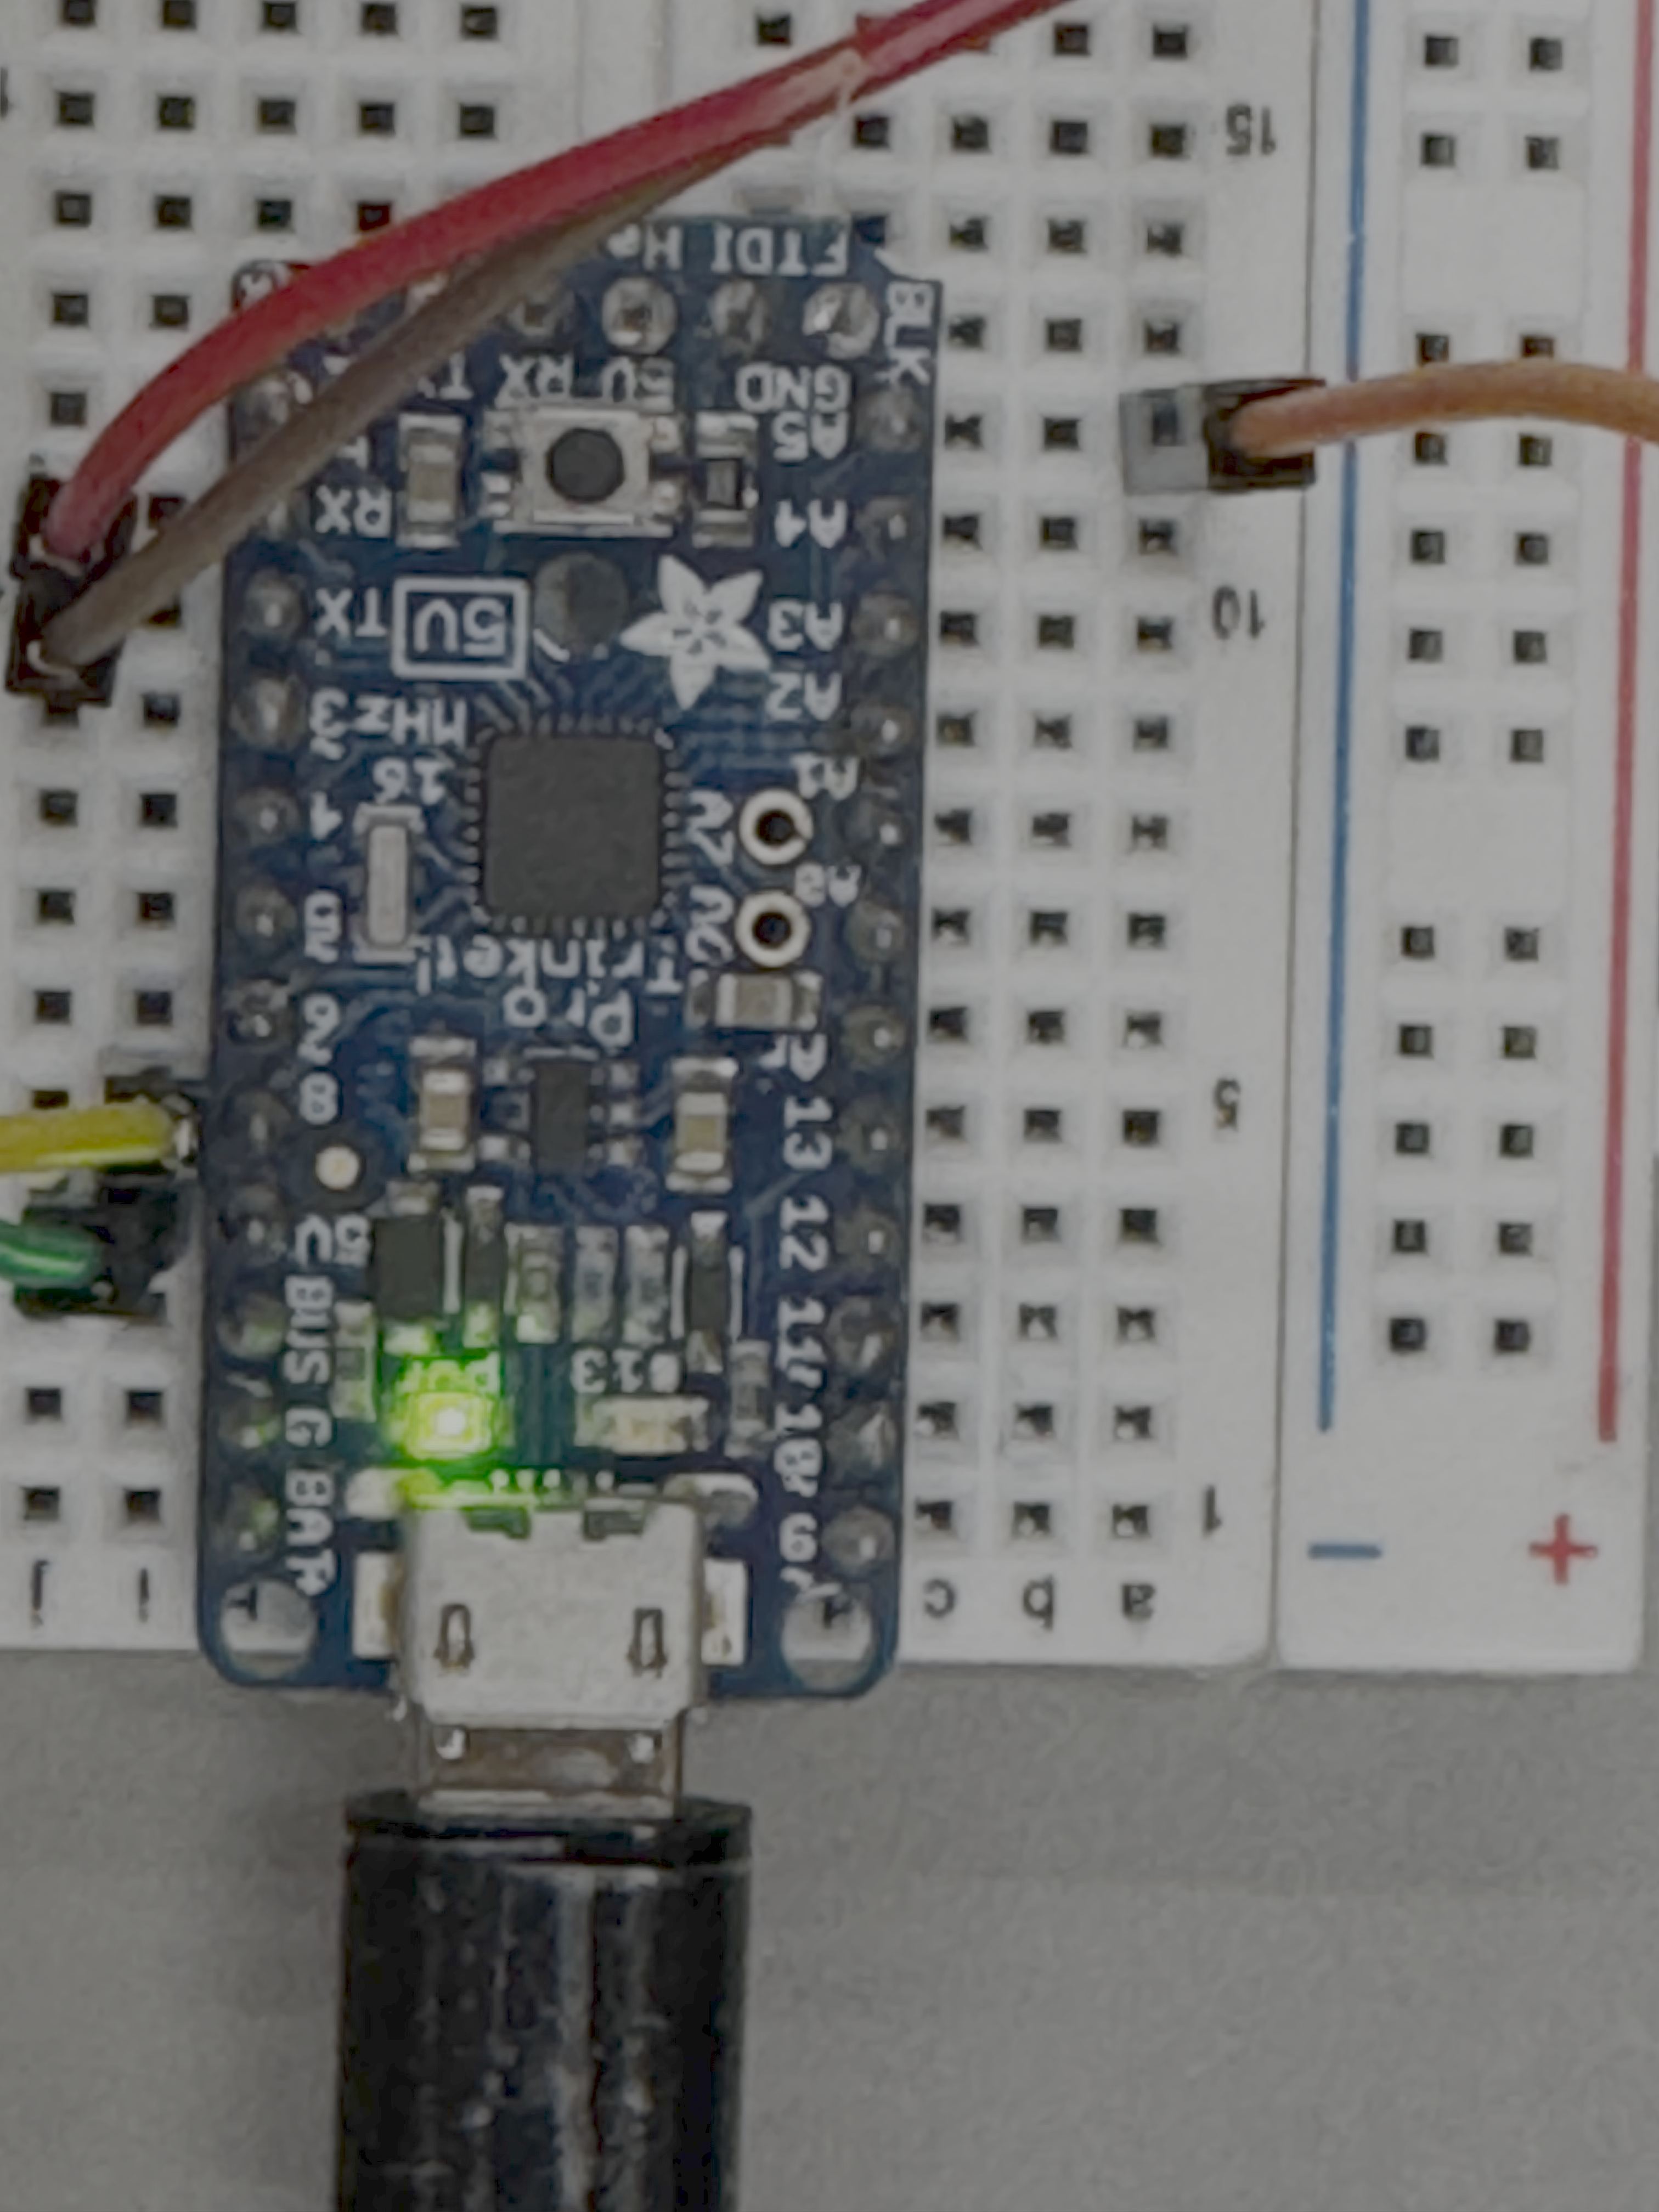
\includegraphics[width=0.85\linewidth]{figures/experiment_hw/board_setup_adfruit_tinkrer_v16mhz_circuit_used_to_attack.png}
  \caption{Pro Tinkrer 5\,V close-up bench setup used for all SCA captures.
           The 10\,$\Omega$ shunt is placed in series with the VCC rail;
           oscilloscope CH1 (differential) measures the voltage drop across
           the shunt proportional to processor current.
           GPIO\,8 is wired to scope CH2 as the hardware trigger.
           The FTDI USB-UART adapter (right) provides the serial plaintext
           channel at 115200\,baud.}
  \label{fig:circuit_trinket}
\end{figure}

\begin{figure}[H]
  \centering
  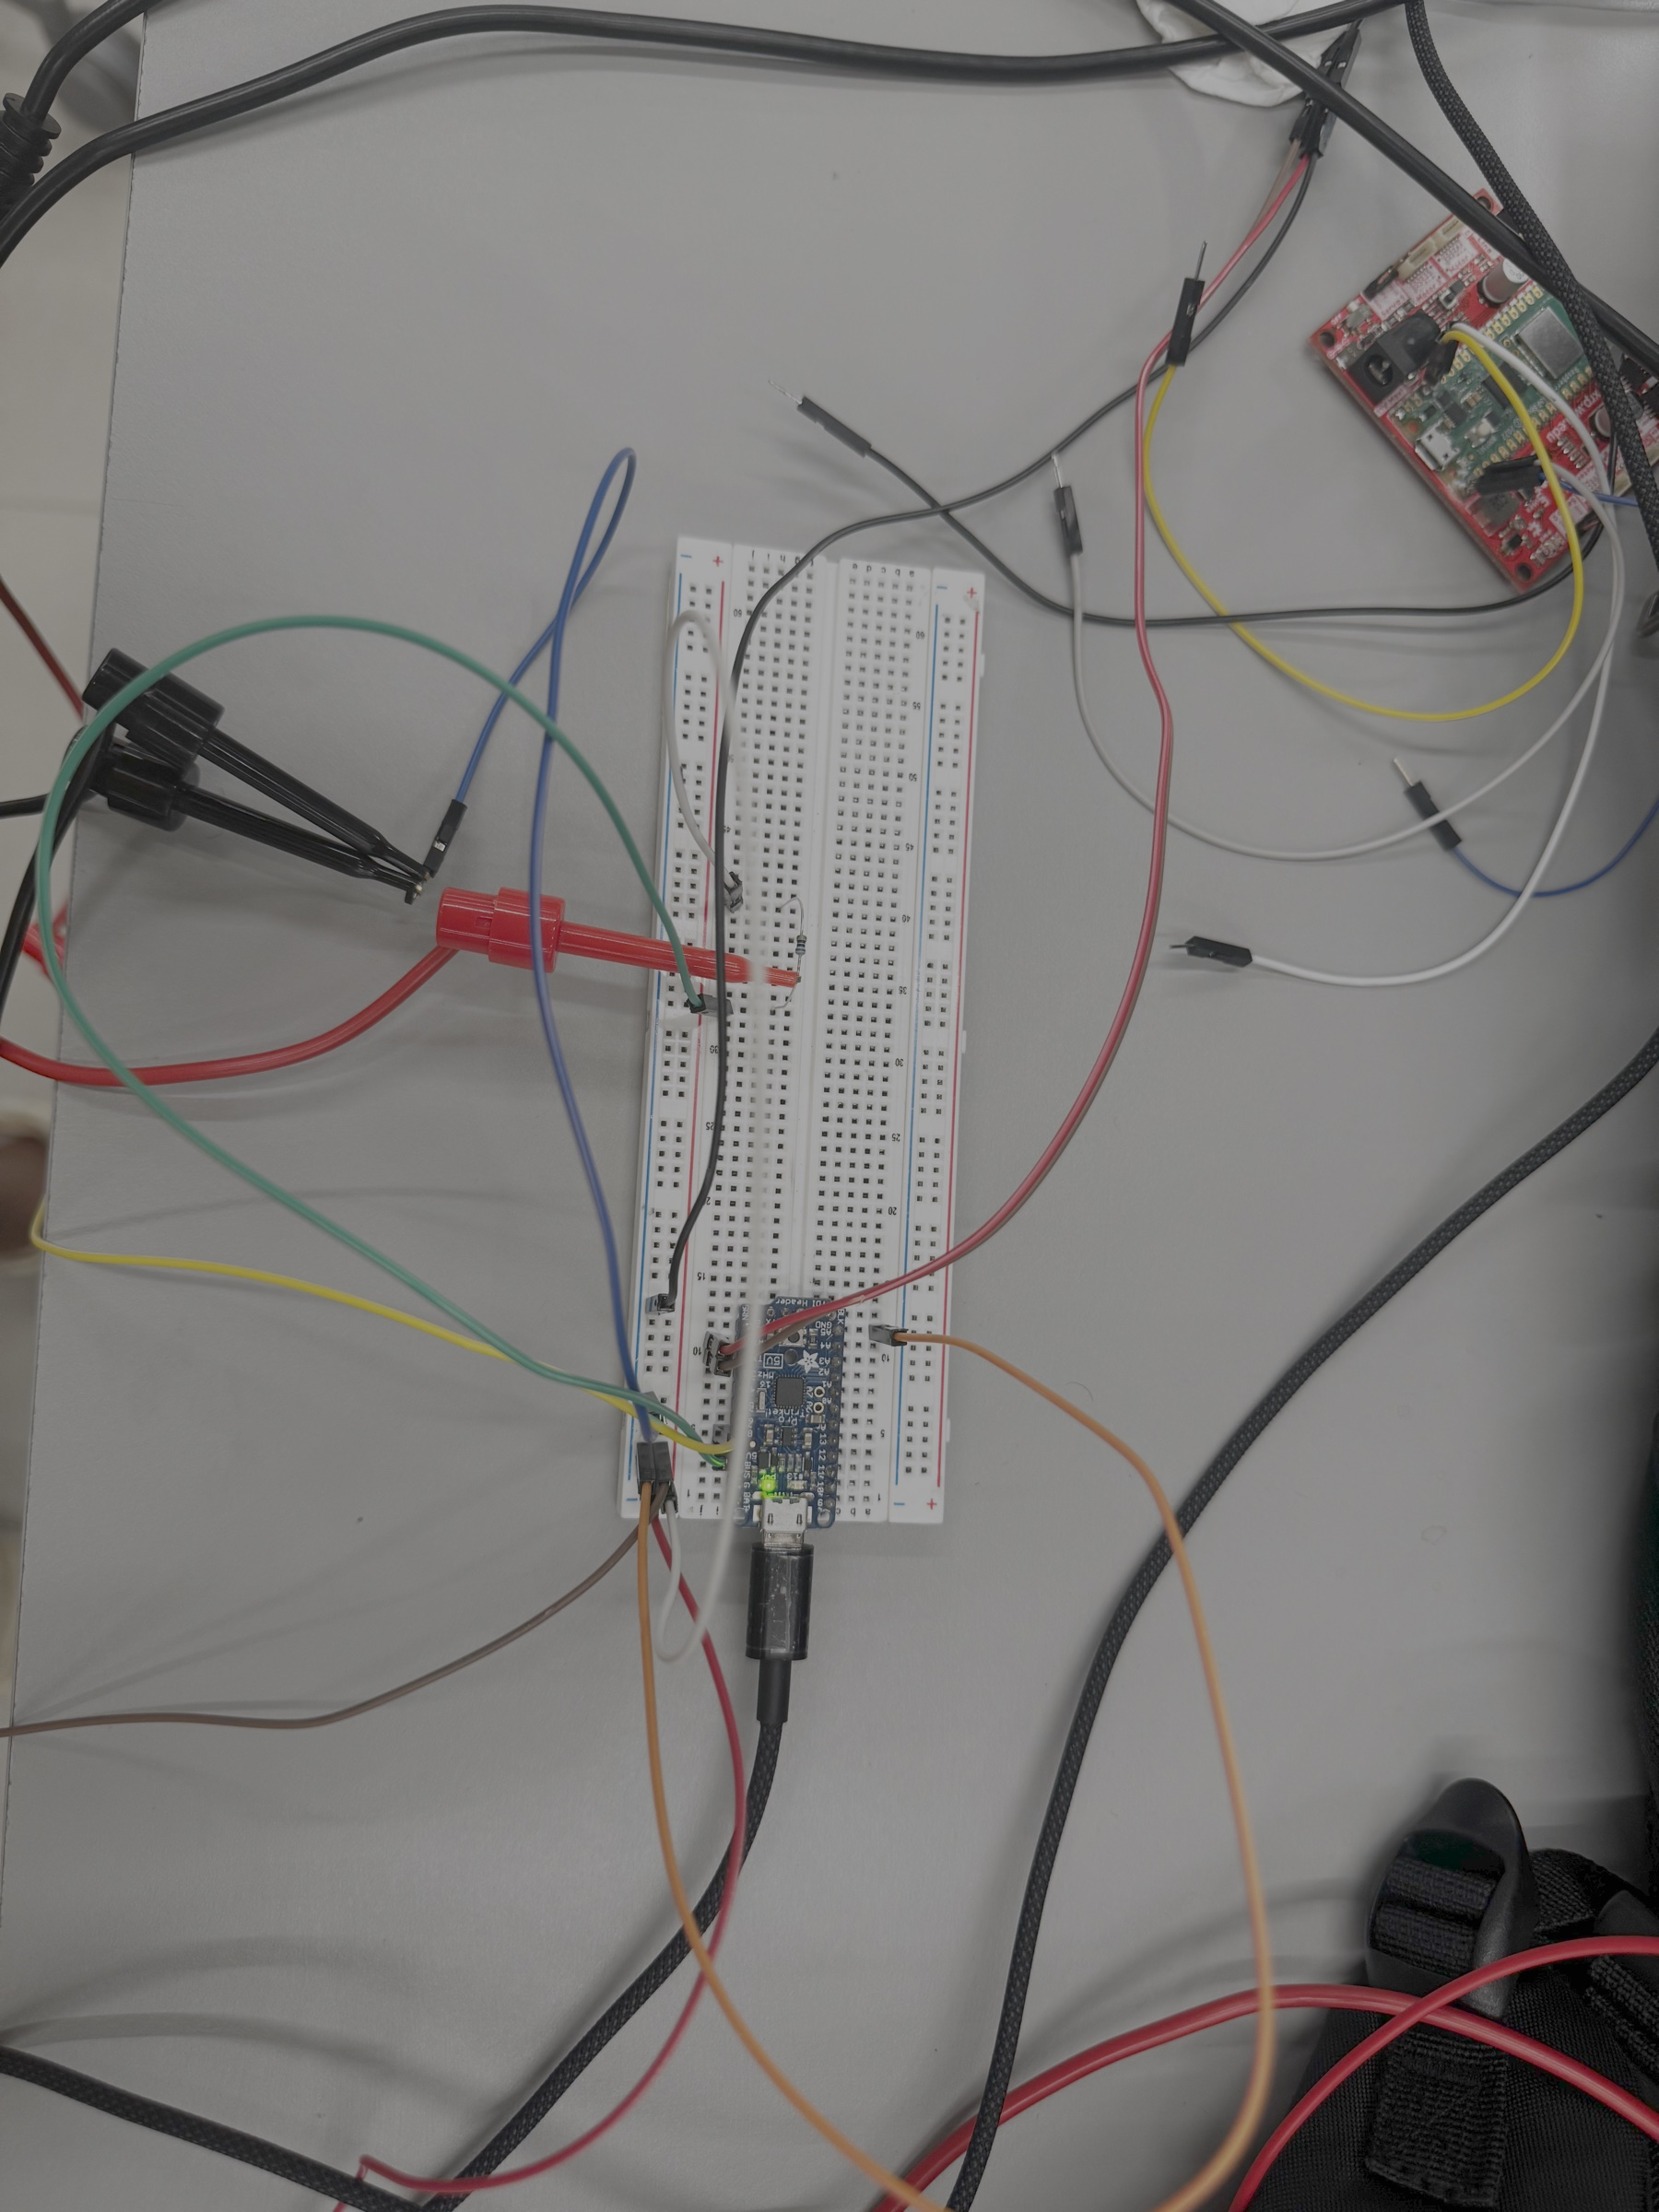
\includegraphics[width=0.85\linewidth]{figures/experiment_hw/full_circuit_picture_detkin_lab.jpg}
  \caption{Full lab bench setup in Detkin Lab.
           Left: Keysight oscilloscope displaying the AES-128 power trace
           on CH1 (differential across 10\,$\Omega$ shunt on VCC rail) and
           the GPIO\,8 hardware trigger on CH2.
           Right: Pro Tinkrer 5\,V with shunt and FTDI USB-UART adapter
           connected to the host capture script.}
  \label{fig:circuit_full}
\end{figure}

% TODO-CIRCUIT-PICO: Insert a photograph of the RPi Pico bench setup.
% Place at report/figures/circuit_pico.jpg and uncomment:
%
% \begin{figure}[H]
%   \centering
%   \includegraphics[width=0.85\linewidth]{figures/circuit_pico.jpg}
%   \caption{RPi Pico RP2040 measurement setup.
%            Shunt placed on GND rail; trigger on GPIO\,22.
%            Attack did not converge due to on-chip SMPS noise
%            (Section~\ref{sec:discussion:hw}).}
%   \label{fig:circuit_pico}
% \end{figure}

\subsection{Video and Photographic Evidence}
\label{app:hw:video}

Video recordings and photographic evidence of the oscilloscope capture
session are hosted in the project repository.
All media links are consolidated in the \textbf{README} under
\emph{Hardware Setup $\to$ Video Demos}:

\begin{center}
  \url{https://github.com/navjotschahal/power_analysis_sca}
\end{center}

The recordings document:

\begin{itemize}
  \item \textbf{Oscilloscope trigger:} GPIO\,8 rising edge firing on the
        Pro Tinkrer , visible on scope CH2.
  \item \textbf{AES power trace:} the first-round AES-128 computation visible
        as elevated switching activity on scope CH1 (differential across
        10\,$\Omega$ shunt).
  \item \textbf{Capture script:} Python acquisition running in terminal with
        \texttt{tqdm} progress bar and per-trace serial latency output.
  \item \textbf{Circuit bench:} Pro Tinkrer with shunt, FTDI adapter, and
        Keysight oscilloscope connections.
\end{itemize}

\noindent
The dataset itself (traces, plaintexts, ciphertexts) is available for
download from Google Drive (link in README):

\begin{center}
  \href{https://drive.google.com/file/d/1Itl82UCQEDyk6cYDD33kB-gKtlXIQBZe/view?usp=sharing}%
       {Google Drive --- Power Trace Dataset (Pro Tinkrer 5\,V, 30{,}000 samples/trace)}
\end{center}
